\section{敏捷软件开发}
敏捷中也有计划驱动

\subsection{敏捷目的}
为了使软件开发团队具有高效工作和快速响应变化的能力

\subsection{敏捷原则}
\vspace{-0.8em}
\begin{multicols}{2}
    \begin{enumerate}[label=\arabic*.]
        \item 最重要的是通过尽早和不断交付有价值的软件满足客户需要
        \item 欢迎需求的变化
        \item 经常交付可以工作的软件,从几星期到几个月,时间尺度越短越好
        \item 业务人员和开发者应该在整个项目过程中始终朝夕在一起工作
        \item 最好的信息传达方式是面对面的交谈
    \end{enumerate}
\end{multicols}
\vspace{-1em}


\subsection{敏捷宣言}
\vspace{-0.8em}
\begin{multicols}{2}
    \begin{itemize}
        \item 个体和互动 胜过 流程和工具
        \item 可以工作的软件 胜过 详尽的文档
        \item 客户合作 胜过 合同谈判
        \item 响应变化 胜过 遵循计划
    \end{itemize}
\end{multicols}
\vspace{-1em}
\vspace{-0.4em}
\begin{itemize}
    \item 也就是说,尽管右项有其价值,我们更重视左项的价值
\end{itemize}

\begin{problem}
请完整描述敏捷宣言。
\end{problem}

\subsection{敏捷软件开发方法}
\subsubsection{极限编程 XP}
eXtreme Programming,极限的含义是指把好的开发实践运用到极致

极限编程的有效实践
\vspace{-0.8em}
\begin{multicols}{2}
    \begin{itemize}
        \item 客户作为开发团队的成员——客户代表
        \item 使用用户素材
        \item 短交付周期
        \item 验收测试
        \item 结对编程——结对编程就是由两名开发人员在同一台计算机上共同编写解决同一个问题的程序代码,通常一个人编码,另一个人对代码进行审查与测试,以保证代码的正确性与可读性。结对编程是加强开发人员相互沟通与评审的一种方式
        \item 测试驱动开发——极限编程强调“测试先行”。在编码之前,应该首先设计好测试方案,然后再编程,直至所有测试都获得通过之后才可以结束工作
        \item 集体所有
        \item 持续集成
        \item 可持续的开发速度 $\leq$40h/week
        \item 开放的工作空间
        \item 重构
        \item 使用隐喻
    \end{itemize}
\end{multicols}
\vspace{-1em}

\subsubsection{Scrum}
迭代式增量软件开发过程:
\begin{figure}[H]
    \vspace{-0.5em}
	\centering
	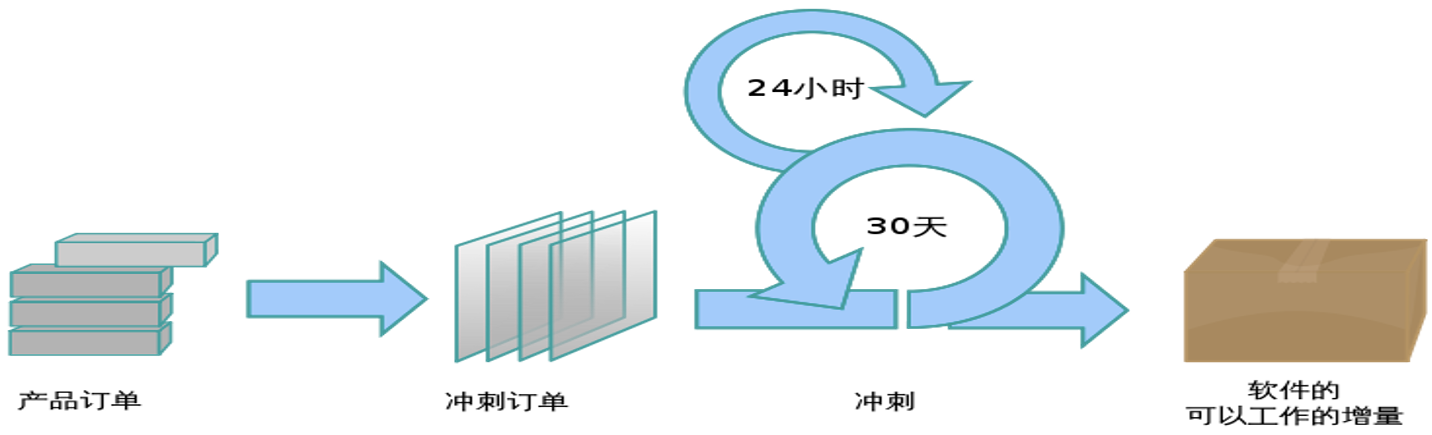
\includegraphics[width=0.65\textwidth]{images/Scrum.png}
    \vspace{-1em}
\end{figure}

Scrum中的文档:
\begin{itemize}
    \item 产品订单(product backlog):整个项目的概要文档,包含了已划分优先等级的、项目要开发的系统或产品的需求清单,是动态的
    \item 冲刺订单(sprint backlog):细化了的文档,包含了团队如何实现下一个冲刺的需求信息
    \begin{itemize}
        \item 哪些产品订单会加入一次冲刺由冲刺计划会议决定。会议中,产品负责人告诉开发团队他们需要完成产品订单中的哪些订单项,开发团队决定在下一次冲刺中承诺完成多少订单项
        \item 在冲刺的过程中,没有人能够变更冲刺订单,这意味着在一个冲刺中需求是被冻结的
    \end{itemize}
    \item 燃尽图(burn down chart)
\end{itemize}

Scrum中角色:
\begin{itemize}
    \item 产品负责人,代表利益所有者
    \begin{itemize}
        \item 产品负责人的职责是将开发团队开发的产品价值最大化
        \item 产品负责人是负责管理产品待办列表的唯一负责人。产品待办列表的管理包括:
        \begin{itemize}
            \item 清晰地表述产品待办列表项
            \item 对产品待办列表项进行排序,使其最好地实现目标和使命
            \item 优化开发团队所执行工作的价值
            \item 确保产品待办列表对所有人是可见、透明和清晰的,同时显示 Scrum 团队下一步要做的工作
            \item 确保开发团队对产品待办列表项有足够深的了解
        \end{itemize}
    \end{itemize}
    \item Scrum Master, 类似于项目经理,负责维护过程和任务
    \begin{itemize}
        \item 促进和支持 SCRUM
        \item 帮助每个人理解 SCRUM 理论、实践、规则和价值
        \item SCRUM Master 是一位服务型领导
        \begin{itemize}
            \item 帮助 SCRUM 团队之外的人了解如何与 SCRUM 团队交互是有益的
            \item 改变SCRUM 团队之外的人与 SCRUM 团队的互动方式来最大化 SCRUM 团队所创造的价值
        \end{itemize}
        \item Scrum Master 服务于产品负责人,包括:
        \begin{itemize}
            \item 确保 Scrum 团队中的每个人都尽可能地理解目标、范围和产品域
            \item 找到有效管理产品待办列表的技巧
            \item 帮助 Scrum 团队理解为何需要清晰且简明的产品待办列表项
            \item 理解在经验主义的环境中的产品规划
            \item 确保产品负责人懂得如何来安排产品待办列表使其达到最大化价值
            \item 理解并实践敏捷性
            \item 当被请求或需要时,引导 Scrum 事件
        \end{itemize}
        \item Scrum Master 以各种方式服务于开发团队,包括:
        \begin{itemize}
            \item 作为教练在自组织和跨职能方面给予开发团队以指导
            \item 帮助开发团队创造高价值的产品
            \item 移除开发团队工作进展中的障碍
            \item 按被请求或需要时,引导 Scrum 事件
            \item 在 Scrum 还未完全采纳和理解的组织环境中,作为教练指导开发团队
        \end{itemize}
        \item Scrum Master 以各种方式服务于组织,包括:
        \begin{itemize}
            \item 带领并作为教练指导组织采纳 Scrum
            \item 在组织范围内规划 Scrum 的实施
            \item 帮助员工和利益攸关者理解并实施 Scrum 和经验导向的产品开发
            \item 引发能够提升 Scrum 团队生产率的改变
            \item 与其他 Scrum Master 一起工作,增强组织中 Scrum 应用的有效性
        \end{itemize}
    \end{itemize}
    \item 开发团队
    \begin{itemize}
        \item 负责在每个 Sprint 结束时交付潜在可发布并且“完成”的产品增量。
        \item 开发团队由组织组建并得到授权,团队自己组织和管理他们的工作。开发团队具有下列特点:
        \begin{itemize}
            \item 他们是自组织的。没有人(即使是 Scrum Master)有权告诉开发团队应该如何把产品待办列表变成潜在可发布的功能增量
            \item 开发团队是跨职能的团队,团队作为一个整体,拥有创建产品增量所需的全部技能
            \item Scrum 不认可开发团队成员的任何头衔,不管其承担何种工作(他们都叫开发人员)
            \item Scrum 不认可开发团队中所谓的“子团队”,无论其需要处理的领域是诸如测试、架构、运维或业务分析
            \item 开发团队中的每个成员也许有特长和专注的领域,但是责任属于整个开发团队
        \end{itemize}
    \end{itemize}
\end{itemize}

Scrum常见活动
\vspace{-0.8em}
\begin{multicols}{3}
    \begin{enumerate}[label=\arabic*.]
        \item Sprint Planning Meeting
        \item Daily standup meeting
        \item review meeting
        \item retrospective meeting
        \item sprint
    \end{enumerate}
\end{multicols}
\vspace{-1em}

Empirical Process Control VS. Statistical Process Control,不同于统计过程控制方法(也叫预测式、计划式)不能解决不可预见的需求变化问题,Scrum采用的实证过程控制承认问题无法完全理解或定义,即用户可以在项目过程中变更需求,关注于如何使开发团队\textbf{快速推出和响应需求变化的能力}最大化


Scrum VS. XP
\begin{itemize}
    \item 迭代周期不同。XP迭代周期为$1\sim 2$周,而Scrum迭代周期为$2\sim 4$周
    \item 迭代中是否允许需求变更。XP中只要变更需求与原需求所需时间资源相等即可变更,而Scrum在迭代中需求被冻结
    \item 迭代中,需求是否严格按照优先级来实现。XP中务必遵守优先级别,Scrum中则比较灵活,原因是可能有需求依赖问题
    \item 过程工程化。Scrum开发过程并未工程化,要求开发者自觉保证,但XP则对开发流程定义严格,例如TDD,结对编程,重构等
\end{itemize}

\subsubsection{Kanban方法}
\vspace{-0.8em}
\begin{multicols}{2}
    \begin{itemize}
        \item 精益生产(丰田制造法)的具体实现
        \item 可视化工作流、限定WIP、管理周期时间
        \item 马丁提出了微服务架构
    \end{itemize}
\end{multicols}
\vspace{-1em}

\subsection{考试题目}
\begin{problem}
	XP规定开发人员每周工作时间不超过\uline{\ \ \ \ \ \ }小时,连续加班不可以超过两周,以免降低生产率?
	\uline{B}    
    \vspace{-0.8em}
    \begin{multicols}{4}
        \begin{enumerate}[label=\Alph*.]
            \item 30
            \item 40
            \item 50
            \item 60
        \end{enumerate}
    \end{multicols}
    \vspace{-1em}
\end{problem}

\begin{problem}
	下列不属于看板方法典型实践的是?
	\uline{BD}    
    \vspace{-0.8em}
    \begin{multicols}{4}
        \begin{enumerate}[label=\Alph*.]
            \item 可视化工作流
            \item 站立式会议
            \item 限定 WIP
            \item 重构
        \end{enumerate}
    \end{multicols}
    \vspace{-1em}
\end{problem}

\begin{problem}
请结合SCRUM这种敏捷方法论述敏捷方法应该具备的特征?同时解释为何常见的若干种描述敏捷方法对立面的方法的特征(例如,严格、重型、计划驱动等等)并不合适?

特征:1. 小周期迭代;2. 快速响应变更;3. 价值交付;4.自动化

特征解释:
\begin{enumerate}[label=\arabic*.]
    \item 严格:所有优秀的工程方法和实践都是严格的
    \item 重型:如上,此外,轻量级和重型其实并没有刻画具体方法,何为重型,并没有严格定义;而且,对于变更这件事情,几乎所有方法都是限制,因此,很难说敏捷方法是轻量级方法
    \item 计划驱动:所有正式的项目都是计划驱动的,否则计划的作用无法体现
\end{enumerate}
\end{problem}

\begin{problem}
敏捷方法的特征有哪些?哪些关于敏捷特征的说法施加于敏捷方法之上是不合适的?为什么?

特征:小周期迭代式、持续交付、敏捷宣言

关于敏捷方法的一些特征表述可能带着一定的误导,例如:
\begin{enumerate}[label=\arabic*.]
    \item 轻量级方法:这是对以XP为代表的一类方法的误导,事实上,这类方法对工程规范有着极为严格的要求
    \item 拥抱变更、变更驱动:仅仅是口号,对待变更,所有软件工程方法都是限制和管理的态度
    \item TDD(测试驱动开发)可以提供更高的开发质量:并没有足够的证据支持
\end{enumerate}
\end{problem}

\begin{problem}
为何说将“规范方法”、“计划驱动方法”等特征作为敏捷方法的对立面带有很大的误导性质?如何通过多种维度改进这种对各类开发过程的理解?

敏捷:敏捷目的、敏捷价值观、敏捷原则

影响敏捷与规范方法选择的五个维度
\begin{enumerate}[label=\arabic*.]
    \item 如果只有强有力的规范而缺乏敏捷,将导致官僚作风,进而停滞不前。团队将陷入为了测量而测量的处境之中,缺乏创新
    \item 缺乏创新的敏捷则如同一个新创公司在盈利之前的不负责任的狂热
    \item 计划驱动的开发人员必须敏捷,敏捷开发人员必须规范
\end{enumerate}
\end{problem}

\begin{problem}
Devops三个步骤
\end{problem}

\begin{problem}
Devops的特点,为什么流行?
\end{problem}

\begin{problem}
什么是云原生?相关的重要的概念
\end{problem}

\begin{problem}
精益屋的两大支柱?
\end{problem}

\begin{problem}
JIT及时生产,价值流和价值拉动的关系
\end{problem}

\begin{problem}
概念解释
\vspace{-0.8em}
\begin{multicols}{3}
    \begin{enumerate}[label=\arabic*.]
        \item CI
        \item CI/CD
        \item Pipeline Orchestration
        \item Container
        \item Micro Service
        \item A/B Testing
        \item GitFlow
    \end{enumerate}
\end{multicols}
\vspace{-1em}
\end{problem}

\begin{problem}
描述用途
\vspace{-0.8em}
\begin{multicols}{5}
    \begin{enumerate}[label=\arabic*.]
        \item Docker
        \item Jenkins
        \item JIRA
        \item SonarQube
        \item Git
    \end{enumerate}
\end{multicols}
\vspace{-1em}
\end{problem}